\chapter{Conclusiones y trabajos futuros}
\fancyhead[R]{8. Conclusiones}


\noindent\fbox{
	\parbox{\textwidth}{
    En este capítulo se tratarán las conclusiones que se han obtenido tras el trabajo, además de detallar las funciones que no se han podido implementar y/o se quieren realizar en un futuro, fuera del contexto del trabajo de fin de grado. También se tratarán los conocimientos y competencias adquiridas durante el desarrollo. 
	}
}


\section{Valoración general del proyecto}

Durante esta sección se hablará de los puntos importantes que se han observado durante la realización de este proyecto, así como los sucesos que han influido en él a la hora de desarrollarlo y las consecuencias que han tenido en tiempos, objetivos y resultados. 

\subsection{¿Qué ha funcionado?}

En general, si bien el desarrollo ha sido un tanto caótico por falta de experiencia en proyectos de esta envergadura, hay multitud de cosas que han funcionado como deberían. Entre ellas a destacar:

\begin{itemize}
    \item \textbf{Investigación y documentación}: El método utilizado para recopilar la información necesaria para este proyecto, iniciando con la búsqueda de conceptos clave y su significado para construir una base, continuando con la lectura y realización de apuntes y anotaciones de términos, técnicas y datos importantes obtenidos de fuentes citadas, y finalizando con la utilización de dicha información para construir las secciones teóricas o prácticas del proyecto, ha sido totalmente satisfactorio. Se ha sentado una base de conocimientos suficientemente útil para no tener que consultar muchas más fuentes tras la investigación inicial, exceptuando la búsqueda de imágenes. 
    \item \textbf{Programación con FreeRTOS y Processing}: La extensa documentación de ambos ha facilitado mucho el desarrollo, además del apoyo de multitud de webs, foros y papers que han utilizado estas tecnologías. En el caso de Processing, el uso de ControlP5 ha agilizado el proyecto por su documentación y ejemplos mostrados en su web, haciendo el desarrollo de la interfaz el doble de rápido de lo que se esperaba en un principio.
\end{itemize}

\subsection{¿Qué errores se han cometido?}

Existen multitud de decisiones que fueron erróneas en un principio, teniendo que corregirlas a posteriori. Aunque la mayoría quedaron solucionados, se han dejado sin cumplir varios objetivos por una mala planificación. Algunos de estos problemas son los siguientes:

\begin{itemize}
    \item \textbf{Componentes}: Al realizar la planificación se intentó tener en cuenta todos los factores que determinaban cuál era el componente correcto, pero algunas variables causaron que se tuviera que comprar otras piezas diferentes, como es el caso de los motores o la maqueta. 
    \item \textbf{Funciones que no se pudieron implementar}: Las funciones relacionadas con el control de la batería, ya nombradas en otros capítulos anteriores, no pudieron realizarse por falta de documentación en ese campo, además de haber subestimado la dificultad y el coste que conllevaban. 
    \item \textbf{Gestión de tiempo}: Aunque se realizó una temporización que, a priori, parecía correcta, los errores y problemas en las diferentes fases de desarrollo han hecho que los plazos no se cumplan en varias secciones, como indica el gráfico posterior en comparación a la figura (pend), mostrada en el capítulo de temporización. Por esta razón se tuvieron que descartar algunas mejoras en la interfaz y el circuito aunque, exceptuando el mayor tiempo de desarrollo, tampoco influyó demasiado en la calidad final del trabajo. 
\end{itemize}


\begin{figure}[h]
    \centering
    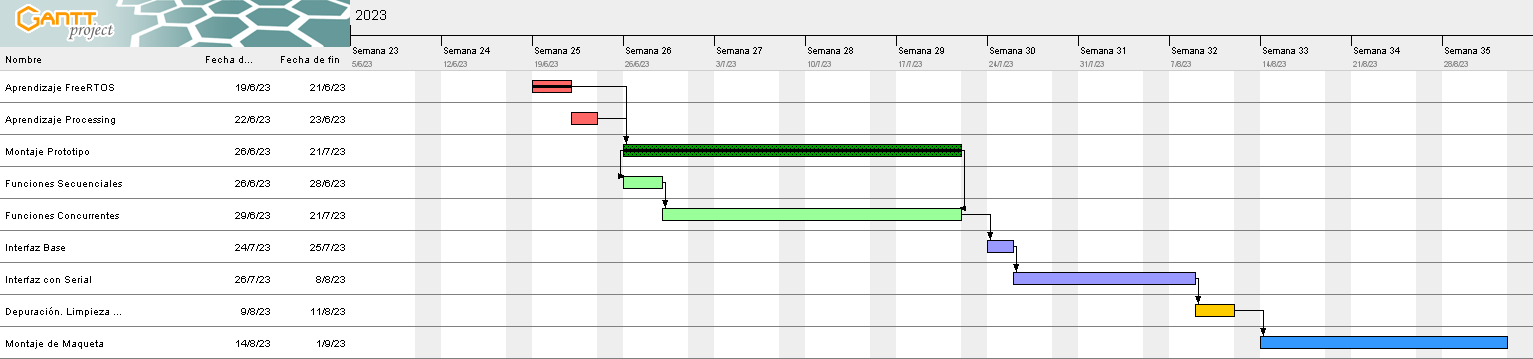
\includegraphics[width=1\textwidth]{imagenes/Gantt_final.png}
    \caption{Diagrama de Gantt con las tareas y su tiempo real de finalización. Elaboración propia en GanttProject}
\end{figure}

\subsection{Objetivos en retrospectiva}

A continuación se detallarán los objetivos que se han cumplido durante el desarrollo, así como aquellos que no se han podido alcanzar debido a las razones comentadas anteriormente. 


\subsubsection*{Objetivos de Investigación}

\begin{itemize}
    \item \textcolor{teal}{\faCheck} \textbf{O-I.1} - Comprender el funcionamiento de una centralita a nivel básico.
    \item \textcolor{teal}{\faCheck}  \textbf{O-I.2} - Sintetizar un conjunto de funciones que podrían ser replicadas en el proyecto.
    \item \textcolor{teal}{\faCheck}  \textbf{O-I.3} - Analizar las alternativas a la hora de implementar los diversos módulos.
    \item \textcolor{teal}{\faCheck}  \textbf{O-I.4} - Conocer los diferentes sistemas del vehículo y cómo interactúan con el entorno mediante sensores y actuadores.
    \item \textcolor{teal}{\faCheck}  \textbf{O-I.5} - Investigar sobre los sistemas de tiempo real y sus limitaciones.
    \item \textcolor{teal}{\faCheck}  \textbf{O-I.6} - Entender las directrices del código propietario y buscar alternativas de código libre para implementar el proyecto.
    \item \textcolor{teal}{\faCheck} \textbf{O-I.7} - Analizar las licencias que se le podrían atribuir al proyecto y escoger una de estas acorde a las características.
    \item \textcolor{teal}{\faCheck} \textbf{O-I.8} - Conocer el impacto de las ECU en el panorama automovilístico actual. 
\end{itemize}

\subsubsection*{Objetivos de Diseño}
\begin{itemize}
    \item \textcolor{teal}{\faCheck}  \textbf{O-D.1} - Diseñar actores y casos de uso para encontrar los límites y soluciones de los que precise el proyecto.
    \item \textcolor{red}{\faRemove}  \textbf{O-D.2} - Diseñar un esquemático para representar cómo interactúan los diferentes módulos con la ECU, así como mostrar los datos que se transmitan.
    \item \textcolor{teal}{\faCheck}  \textbf{O-D.3} - Programar la ECU para la recepción, tratamiento y envío de datos.
    \item \textcolor{teal}{\faCheck}  \textbf{O-D.4} - Implementar una interfaz de usuario para poder mostrar los módulos que buscamos.
    \item \textcolor{teal}{\faCheck}  \textbf{O-D.5} - Recrear este sistema en una maqueta de manera física si la temporización lo permitiera.
\end{itemize}

\section{Trabajos futuros}

Una vez finalizado el trabajo, y ya como desarrollo personal o por hobby, se intentarán implementar aquellas funciones que tienen que ver con la batería, además de perfeccionar el proyecto y añadir otras funcionalidades que puedan ser interesantes. También se trabajará en hacer el módulo inalámbrico, únicamente alimentado por baterías, con una comunicación bluetooth. 

\section{Competencias y conocimientos adquiridos}

Con la realización de este trabajo se han adquirido conocimientos y habilidades en multitud de campos, además de consolidar aquellos obtenidos durante la carrera en múltiples asignaturas. Si bien el grueso de lo aprendido pertenece al área del hardware y la ingeniería de computadores, con la construcción del circuito, elección de componentes, y programación de un sistema empotrado con un RTOS, también se han utilizado conocimientos de otros campos estudiados. Algunos de estos son relativos a la rama de Ingeniería del Software, como puede ser la creación de la interfaz de usuario e ingeniería de requisitos, así como también se ha utilizado la base de electrónica para calcular voltajes, resistencias y estructura del circuito en general. 

Ha sido un primer contacto muy educativo con los sistemas de tiempo real y las interfaces de usuario, temas que, si bien se habían comentado de manera superficial en algunas asignaturas cursadas, nunca se habían profundizado al nivel que se ha alcanzado en este trabajo. También el manejo del tiempo, la planificación y la constancia han hecho que, de ahora en adelante, sea más sencillo iniciar un proyecto a este nivel, ya sea por simple interés o \textit{hobby}, o por necesidad en el futuro laboral. 

\section{Experiencia personal}

Después de todos estos meses trabajando en el proyecto, con sus altos y sus bajos, no puedo estar mucho más contenta de lo que estoy con lo que se ha conseguido. Al comienzo fue difícil, pues no sabía cómo empezar a escribir, cómo organizar todo el trabajo, ni cuánto tiempo iba a llevar. Han pasado ya unos meses desde que le presenté la idea al tutor, y desde ahí en adelante cada vez se ha hecho más sencillo abordar las distintas secciones que conforman el trabajo. Ha sido una experiencia gratificante y agobiante a partes iguales, pero me quedo con todo lo que he aprendido y mejorado en todos los sentidos. 